\documentclass[10pt]{article}
\usepackage[margin=0.7in,top=0.55in,bottom=0.55in]{geometry}
\usepackage{amsmath,amssymb,booktabs,microtype,xcolor,url,graphicx}
\usepackage[colorlinks=true,linkcolor=blue!60!black,urlcolor=blue!60!black,pdftitle={FRE-GY-9743 Assignment 7},pdfauthor={Raj Pawar}]{hyperref}
\newcommand{\code}[1]{\texttt{#1}}
\setlength{\parindent}{0pt}\setlength{\parskip}{3pt}\emergencystretch=3em\pagestyle{plain}
\makeatletter\g@addto@macro\normalsize{\setlength{\abovedisplayskip}{5pt}\setlength{\belowdisplayskip}{5pt}\setlength{\abovedisplayshortskip}{3pt}\setlength{\belowdisplayshortskip}{3pt}}\makeatother
\makeatletter\renewcommand{\section}{\@startsection{section}{1}{\z@}{8pt plus 2pt}{3pt}{\normalfont\large\bfseries}}\makeatother
\begin{document}
{\Large\bfseries FRE-GY-9743 Assignment 7: A Monotone Convex Interpolator for the IFR Curve}\\[1pt]
Raj Pawar, NYU Tandon School of Engineering, November 14, 2026.\\
Code: \href{https://github.com/pawarraj8888/FRE-GY-9743-Assignments-7/tree/Raj_Pawar_Branch}{github.com/pawarraj8888/FRE-GY-9743-Assignments-7}, branch \code{Raj\_Pawar\_Branch}.\\
Implementation: class \code{Interpolator1DMonotoneConvex} in \code{fixedincomelib/utilities/numerics.py}.\\
Project page: \href{https://pawarraj8888.github.io/FRE-GY-9743-Assignments-7/}{pawarraj8888.github.io/FRE-GY-9743-Assignments-7}.
\vspace{2pt}\hrule

\section*{1. What the curve has to do}
The yield-curve model stores each index as an instantaneous forward rate (IFR) curve $f(t)$ through node times $0<t_0<\dots<t_n$
(ACT/ACT years from the value date) with node values $f_0,\dots,f_n$, and discounts with $D(T)=\exp\bigl(-\int_0^T f(s)\,ds\bigr)$.
The library ships a left-continuous piecewise constant curve (PCP): on $(t_{i-1},t_i]$ it uses $f_i$, the value at the \emph{right} end
of the interval. The mini project asks for a curve that passes through the supplied points, is continuous, and is monotone and convex
within each node interval whenever the data allow it, with flat extrapolation and a one-node curve that is constant; only
\code{interpolate} and \code{integrate} are needed, and the two optional gradient stubs stay as supplied. Monotone and convex inside
an interval means the curve can neither overshoot an endpoint nor wiggle between the two, so the forward rates, and with them every
ratio of discount factors, carry nothing that is not in the data.

\section*{2. The method}
\textbf{Point values, not interval averages.} Hagan and West build their monotone convex curve from discrete forwards $f^d_i$ that
belong to whole intervals: the node values $f_i$ are free (the linear interpolation of the two neighbouring interval averages) and each
piece is a quadratic in $g=f-f^d_i$ whose integral is pinned to zero. Here the node values are the data, so the free quantities are the
node slopes $d_i=f'(t_i)$, and the integral over an interval is an output. I kept their structure (local estimates at the nodes, one
or two quadratics per interval, a flat segment inserted where the plain quadratic would break monotonicity) and moved it one derivative up.

\textbf{Step 1: node slopes.} With $h_i=t_i-t_{i-1}$ and chord slopes $s_i=(f_i-f_{i-1})/h_i$ for $i=1,\dots,n$, an interior node gets
\[
d_i=\begin{cases}0 & \text{if } s_i\,s_{i+1}\le 0,\\[3pt] \dfrac{w_1+w_2}{w_1/s_i+w_2/s_{i+1}} & \text{otherwise},\end{cases}
\qquad w_1=2h_{i+1}+h_i,\quad w_2=h_{i+1}+2h_i,
\]
the weighted harmonic mean of Fritsch and Butland, and $|d_i|$ is then capped at $2\min(|s_i|,|s_{i+1}|)$. At the two ends I take the
slope of the parabola through the three outermost points, $d_0=\bigl((2h_1+h_2)\,s_1-h_1s_2\bigr)/(h_1+h_2)$ and its mirror image at
$t_n$, set to zero when its sign disagrees with the end chord and capped at twice that chord. Three facts follow directly: (P1) every
$d_i$ is zero or has the sign of the chords on both sides of its node; (P2) an interior $d_i$ lies between $s_i$ and $s_{i+1}$, because
a weighted harmonic mean of two numbers of one sign does; (P3) $|d_i|\le 2\min(|s_i|,|s_{i+1}|)$, $|d_0|\le 2|s_1|$ and $|d_n|\le 2|s_n|$.
With two nodes both slopes equal the chord and the curve is the straight line; with one node it is the constant.

\textbf{Step 2: the piece on $[t_{i-1},t_i]$.} I make $f'$ piecewise linear through $(t_{i-1},d_{i-1})$, $(\xi,m)$ and $(t_i,d_i)$,
with one knot $\xi=t_{i-1}+\alpha$ and $\beta=h_i-\alpha$. The curve is then two quadratics joined with a continuous derivative, and it
lands exactly on $f_i$ when the derivative integrates to $f_i-f_{i-1}$, that is when
$m=2s_i-(\alpha d_{i-1}+\beta d_i)/h_i$. Write $a=s_i-d_{i-1}$ and $b=d_i-s_i$ for the end slopes measured from the chord.
\begin{itemize}\setlength{\itemsep}{1pt}\setlength{\topsep}{2pt}
\item $ab>0$: the end slopes straddle the chord. Following Schumaker's shape-preserving quadratic spline I place the knot where one of the
two pieces becomes a straight line: if $|b|\le|a|$ then $\alpha=2h_i|b|/(|a|+|b|)$ and $m=d_i$ (the right piece is linear with slope
$d_i$), otherwise $\alpha=h_i(|b|-|a|)/(|a|+|b|)$ and $m=d_{i-1}$ (the left piece is linear); when $|a|=|b|$ a single quadratic does it.
Either way $f'$ moves monotonically from $d_{i-1}$ to $d_i$, so the piece is convex when $a,b>0$ and concave when $a,b<0$, and by (P1)
all three slopes carry the sign of the chord, so the piece is monotone. This linear segment is the slope-space version of Hagan and
West's flat segment.
\item $ab\le 0$ and not both zero: both end slopes sit on the same side of the chord, or one equals it. No $C^1$ convex or concave piece
exists, because a derivative that moves monotonically from $d_{i-1}$ to $d_i$ cannot average to $s_i$. I put the knot at the midpoint,
$m=2s_i-\tfrac12(d_{i-1}+d_i)$; by (P3) $|d_{i-1}|,|d_i|\le 2|s_i|$, so $m$ has the sign of $s_i$ or is zero, and the piece is still
monotone, with one inflection.
\item $a=b=0$: the straight line.
\end{itemize}
The implementation stores the breakpoints, the three coefficients of every quadratic and the running integral at each breakpoint, so
\code{interpolate} is a binary search plus one quadratic and \code{integrate}$(a,b)$ is the difference of two antiderivative values;
outside $[t_0,t_n]$ the curve is flat at $f_0$ and $f_n$.

\textbf{Which data are compatible, and what happens otherwise.} If the chord slopes do not decrease across an interval,
$s_{i-1}\le s_i\le s_{i+1}$, then by (P2) $d_{i-1}\le s_i\le d_i$, so $a,b\ge0$ and the piece is monotone and convex (concave data give
a monotone concave piece). Both supplied curves are of this kind: the SOFR chords rise from 0.20\% to 0.60\% per year and the Fed
Funds chords from 0.14\% to 0.50\%, so every interval is monotone and convex, which the notebook confirms by checking first and
second differences on a 2000-point grid in each of the five intervals of both curves. Data can be incompatible in two ways. At a local
extremum of the data the slope at that node is zero, so the peak or trough sits at the node, nothing overshoots, and the curve is smooth
there; the two adjacent pieces are concave (a hump) or convex (a bowl). A convex piece on both sides of a maximum is only possible with
a kink, and this is where I choose smoothness over convexity. At a node where the data turn from convex to concave the slope rule still
gives a $C^1$ monotone curve, but one of the neighbouring pieces carries an inflection. So monotonicity, continuity and a continuous
derivative hold for any data, and convexity holds exactly on the intervals whose data are locally convex. Positivity is inherited from
the data, since the curve never leaves the range of its two endpoint values. Flat extrapolation beyond $t_n$ meets a rising convex last
piece with a kink (the slope drops to zero), the counterpart of the jump that PCP has there; a zero end slope in the Hagan and West manner
would remove the kink but would make the last piece concave, which the brief rules out.

\textbf{Locality and stability.} A node value enters only its own slope and the slopes of its two neighbours, so a change at $f_i$ moves
the curve on at most the four intervals between $t_{i-2}$ and $t_{i+2}$, as in the unameliorated Hagan and West method. The harmonic mean
and the cap keep every slope within twice the smaller adjacent chord, so a short steep interval cannot drag the curve next to it; this
is the role their positivity collar $f_i\le 2\min(f^d_i,f^d_{i+1})$ plays.

\section*{3. Results}
\begin{center}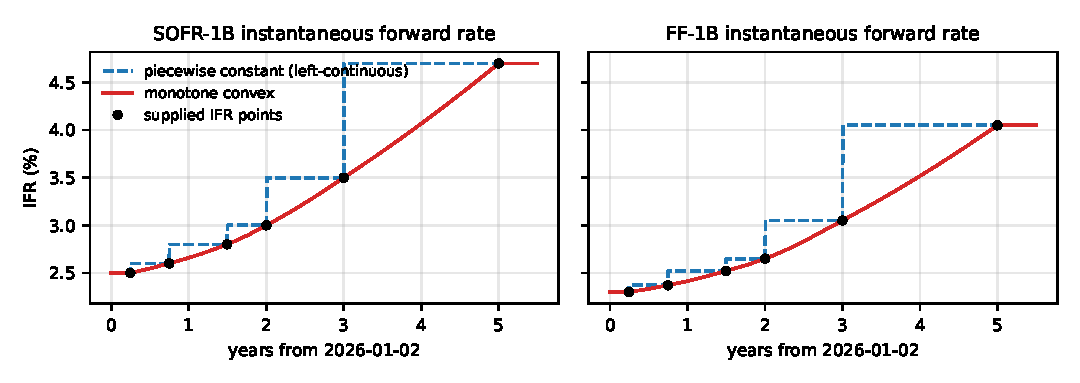
\includegraphics[width=\textwidth]{ifr_curves.pdf}\end{center}
\vspace{-6pt}
{\small Figure: the two index curves under the supplied piecewise constant interpolation and under mine (value date 2026-01-02, flat
extrapolation on both sides). The funding curve has one node, 5 bp over SOFR, and is the same constant under both.}

\begin{center}\footnotesize
\begin{tabular}{@{}lrrr@{}}\toprule
Product (notebook cells, notional 1,000,000) & PCP PV & Monotone convex PV & Difference \\ \midrule
FRA, 2026-05-05 to 2026-11-05, receive 3.2\% & 2,908.29 & 3,261.84 & 353.56 \\
RFR swap, 2026-04-02 to 2029-04-02, receive 3.4\% annual & 6,222.52 & 12,874.70 & 6,652.19 \\
Overnight basis swap, 2026-07-02 to 2028-07-03, receive SOFR + 10 bp, pay FF & 8,351.35 & 7,631.94 & -719.41 \\
\bottomrule\end{tabular}\end{center}

\textbf{Why the PVs move.} PCP uses $f_i$ on the whole interval that ends at $t_i$, so on rising data the step sits above the point
curve everywhere (figure); my curve passes through the points and, being convex, stays below each chord. Floating legs are therefore
smaller, discount factors slightly larger, and a receiver of fixed gains. \emph{FRA:} the forward for 2026-05-05 to 2026-11-05 drops from
2.6182\% to 2.5478\%, because PCP holds 2.6\% from 2026-04-02 onwards while my curve climbs from 2.5\% to 2.6\% over that interval;
$10^6\times\alpha\times(K-F)\times D$ with $\alpha=0.5111$ gives 3,261.84 against 2,908.29. \emph{Swap:} the three compounded annual
SOFR rates fall from 2.699\%, 3.077\%, 3.809\% to 2.601\%, 2.902\%, 3.370\%. The last one moves most: after the 3Y node PCP jumps
straight to the 5Y value of 4.7\% while my curve is still at 3.5 to 3.6\% (it averages 3.57\% over the final quarter), so the floating
leg falls from 90,552.57 to 84,240.04 while the fixed leg rises from 96,775.08 to 97,114.75 through the discount factors.
\emph{Basis swap:} I receive SOFR plus 10 bp and pay Fed Funds, so what matters is the SOFR--FF gap. PCP's gap over the seven regular
quarters is the right-node gap, 27.8, 27.8, 28.1, 34.8, 34.8, 44.6, 44.6 bp; my curves pass through the point gaps (20, 23, 28, 35, 45 bp at the nodes) and give
23.6, 25.1, 26.8, 29.4, 33.0, 36.2, 38.8 bp over the same quarters, so the leg difference shrinks from 8,351.35 to 7,631.94 even though both legs fall by about
3,000 (59,485.39 and 51,134.04 become 56,411.56 and 48,779.61).

\section*{4. Checks and notes}
\textbf{Tests.} \code{tests/test\_monotone\_convex\_interpolator.py} has 22 tests: the one-node and two-node curves, interpolation
through the points, continuity and a continuous derivative at every breakpoint, the slope rules (sign, bounds, zero at an extremum, the
cap binding on a short steep interval next to a long flat one), monotone and convex pieces on rising, falling, concave, hump and bowl
data, the midpoint-knot case with its inflection, 50 random data sets that never overshoot, \code{integrate} against Simpson quadrature
of \code{interpolate}, additivity and sign, flat extrapolation, a three-node curve worked out by hand (slopes $7/6$, $9/13$, $1/6$, knot
positions and integrals), the model's discount factors, a 1 bp bump of one node that only moves the curve near it, and the six notebook
PVs. The build also re-derives the six PVs in plain Python from a second implementation of the recipe and hand-written schedules.

\textbf{Risk.} The gradient stubs stay as supplied, as the notebook asks. The curve is a nonlinear function of the node values (the
harmonic mean and the knot position both depend on them), so an ordinate gradient would need the derivative of the slope rule; since
\code{perturb\_model\_parameter} rebuilds the interpolator, bump-and-reprice risk works with no further change.
\end{document}
